\section{ฟังก์ชันของการแปรผันที่มีขอบเขต}

\hspace{1cm} ให้ $\Omega$ เป็นเซตเปิดที่มีขอบเขตของ $ \mathbb{R}^{d}$ และให้ $u \in L^{1}(\Omega)$ เรานิยามการแปรผันรวม (total variation) ของ $u$ เป็น
\begin{align} 
    \int_{\Omega} |Du| = \text{sup} \Big\{ \int_\Omega u \nabla \cdot \mathbf{\varphi} d \mathbf{x} | \mathbf{\varphi} = (\varphi_1, \varphi_2, ... , \varphi_d) \in C_0^1 (\Omega, \mathbb{R}^d )^d \\
    \nonumber \text{ และ } || \phi_i ||_{L^{\infty}} \leq 1 \text{ สำหรับ } i = 1,..., d  \Big\}
\end{align}

%$\nabla \cdot \varphi = \sum_{i=1}^{d} \frac{\partial \varphi_i}{\parital x_i} $,

เมื่อ $\nabla \cdot \varphi = \displaystyle \sum_{i=1}^{d} \frac{\partial \varphi_i}{\partial x_i (\mathbf{x})}$, $d \mathbf{x}$ เป็น Lebesgue measure และ $C_0^1 ( \Omega , \mathbb{R}^d)$ คือปริภูมิของฟังก์ชันต่อเนื่องที่หาอนุพันธ์ได้และกระชับใน $\Omega$

\hspace{1cm}ถ้า $u \in C_0^1 (\Omega, \mathbb{R}^d )$ จะได้
\begin{align}
    \int_\Omega u \nabla \cdot \varphi d x = - \int_\Omega \sum_{i=1}^{d} \frac{\partial u}{\partial x_i} \varphi_i d \Omega
\end{align}

สำหรับทุก $\varphi \in C_0^1 (\Omega,\mathbb{R}^{d})^{d} $ ดังนั้น
\begin{align}
    \int_\Omega | D u | = \int_\Omega | \nabla u | dx
\end{align}

\hspace{1cm}ฟังก์ชัน $u \in L^1 (\Omega)$ เรียกว่าฟังก์ชันที่มีการแปรผันแบบมีขอบเขตใน $\Omega$ และจะใช้สัญลักษณ์ $BV(\Omega)$ แทนปริภูมิของทุกๆ ฟังก์ชันใน $L^1(\Omega)$ ที่มีการแปรผันแบบมีขอบเขต
\begin{Example}
    ฟังก์ชัน $f1, f2 \text{และ} f3 $ ซึ่งกำหนดโดย
    \begin{align}
        f1(x) = \sin{(x)},
    \end{align}
    \begin{align}
        f2(x) = \left\{
            \begin{array}{ll}
              1/4, \hspace{1cm}  &x \in [0,\pi/8] \\
              1/2, \hspace{1cm}  &x \in [\pi/8,\pi/4] \\
              3/4, \hspace{1cm}   &x \in [\pi/4,3\pi/8] \\
              1,   \hspace{1cm} &x \in [3\pi/8,\pi/2] \\
            \end{array}
          \right.
    \end{align}
    \begin{align}
        f3(x) = \frac{2x}{\pi},
    \end{align}
    เป็นฟังก์ชันในปริภูมิ $BV(\Omega)$ ถ้า $\Omega = [0, \pi/2]$ และทั้ง 3 ฟังก์ชันด้านบนการแปรผันรวมเดียวกันคือ 1 สำหรับฟังก์ชัน $f4$ กำหนดโดย
    \begin{align}
        f4(x) = \left\{ 
            \begin{array}{ll}
                0,  \hspace{1cm}  &  x = 0 \\
                \sin (1/x),  \hspace{1cm}  & x \in (0,a) \text{ และ } a > 0
            \end{array}
        \right.
    \end{align}
    
    มีการแปรผันรวมอนันต์ (infinite total variation) และไม่อยู่ในปริภูมิ $BV(\Omega)$ ซึ่ง $\Omega = [0,a]$ สำหรับทุก $a > 0$
    \begin{figure}[H]
	\centering
	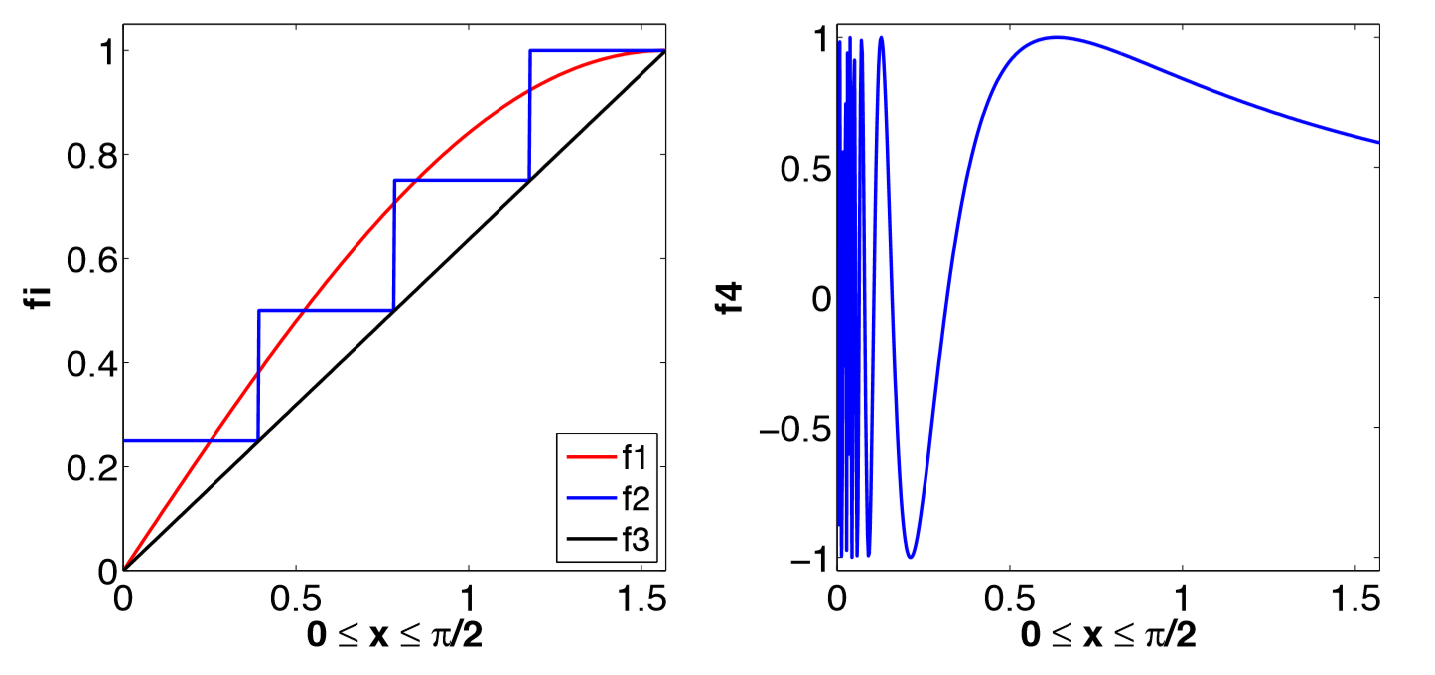
\includegraphics[width=0.8\linewidth]{image/boundary_condition/function_slove.png}
	\caption{ฟังก์ชันแปรผันมีขอบเขตทั้งสามฟังก์ชันที่มีการแปรผันรวมเหมือนกันเท่ากับ 1  และฟังก์ชันที่มีการแปรผันไม่จำกัด}
	\label{figure:sample-domain}
\end{figure}
\end{Example}
